\documentclass[12pt]{article}

\usepackage{sbc-template}
\usepackage{graphicx,url}
\usepackage[latin1]{inputenc}  

\usepackage{../Utils}
\usepackage{implementation}     
\sloppy

\title{The Implementation of Proxima \\{\small \version}}

\author{Martijn M. Schrage\inst{1}}


\address{Institute of Information and Computing Sciences\\ Utrecht University\\
    Utrecht, The Netherlands
  \email{martijn@cs.uu.nl}
}

\begin{document} 

\maketitle

\begin{abstract}

\end{abstract}
     
\bc

Introduction (2)

Proxima's layered architecture (2)
- explanantion of presentation/interpretation processes
- overview of levels and layers
  (much can be taken from thesis chapter)
  
Presentation process
  
  Xprez (2)
  - short version of thesis chapter
  Presentation (2)
  - explanation of AG system
  - structural vs parsing
  - examples
   
Interpretation process 
  Scanner (2)
  - regular expression for specifying tokens
  - example
 
  Parser  (2)
   - structural vs parsing
   - uuag parser with only a few extra things
   - example
  Error handling in parser and scanner
 
Related work (1/2)
- synthesizer generator
- eclipse
- barista

Conclusions (1/2)

\ec

\section{Introduction}

\bl
\o what is Proxima~\cite{schrage04Proxima}.
\o modeless combination of structure editing and free editing in the presentation
\o nothing is primitive
\o example applications
\o Editor for Baysian networks
\o Generic editor as IDE
\o by giving type, pres, and parser, we get an environment almost for free
\o Helium editor
\o Implementation of Proxima
\o overview of paper 
\el

\begin{figure}[ht]
\centering
\includegraphics[width=\textwidth]{images/screenshots/BayesDocEditor}
\caption{The Bayesian network documentation editor}
\label{fig:bayesEditor}
\end{figure}


%%%%%%%%%%%%%%%%%%%%%%%%%%%%%%%%%%%%%%%%%%%%%%%%%%%%
%
\section{Proxima's layered architecture} \label{sec:architecture}
%
%%%%%%%%%%%%%%%%%%%%%%%%%%%%%%%%%%%%%%%%%%%%%%%%%%%%

The core architecture of Proxima consists of a number of layers, which only communicate with their direct neighbors. This layered structure is based on the staged nature of the presentation process. Instead of mapping a document directly onto its final rendering, it is first mapped onto an intermediate data structure. This intermediate data structure is mapped onto another intermediate data structure, until the last intermediate data structure is mapped onto the rendering.

As we mentioned in Chapter~\ref{chap:introduction}, the positions at which the document, the rendering, and the intermediate data structures reside are called {\em data levels}. Between each pair of levels is a {\em layer}, which is a component that maintains the mappings between the levels. Figure~\ref{proxlayers} schematically shows the levels and layers of Proxima. Only two data levels are visible to each layer: a higher and a lower level.

\begin{figure}[ht]
\centering
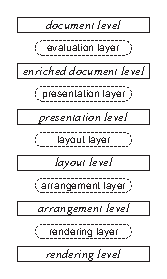
\includegraphics[width=4cm]{images/LevelLayerNames}
\caption{The Bayesian network documentation editor}
\label{fig:bayesEditor}
\end{figure}


A data level in Proxima is not just an intermediate value in the presentation computation, but an entity in its own right. Together, the data levels constitute the state of the editor. The six data levels of Proxima are:


\begin{description}
\item[Document:] The edited document, the type of which is specified by a DTD or an EBNF grammar.

\item[Enriched Document:] The document enriched with computed information.

\item[Presentation:] A logical description of the presentation of the document, consisting of rows and columns of presentation elements with attributes. The presentation also supports formatting based on available space (e.g.\ line/page breaking).

\item[Layout:]  Presentation with explicit whitespace.

\item[Arrangement:] Formatted presentation with absolute size and position information.

\item[Rendering:] A collection of user interface commands for drawing the absolutely positioned and sized arrangement.
\end{description}



\bl
\o explain why layered
\o overview of layers
\o explain choice of layers
\o explain where actual editing takes place
\o and skipping of layers
\o implementation: layer combinators.
\o sometimes awkward, because we have to conform to the layers.
\o but this has advantages: new GUI lib in a matter of days.
\el




%%%%%%%%%%%%%%%%%%%%%%%%%%%%%%%%%%%%%%%%%%%%%%%%%%%%
%
\section{The document structure}
%
%%%%%%%%%%%%%%%%%%%%%%%%%%%%%%%%%%%%%%%%%%%%%%%%%%%%

\bl
\o Document is main data type
\o Haskell types, no parameters
\o fields to store token id's for handling whitespace and focus
\o holes and parse errors added to each nonterminal
\el




%%%%%%%%%%%%%%%%%%%%%%%%%%%%%%%%%%%%%%%%%%%%%%%%%%%%
%
\section{The {\Xprez} presentation language} \label{sect:xpreztarget}
%
%%%%%%%%%%%%%%%%%%%%%%%%%%%%%%%%%%%%%%%%%%%%%%%%%%%%



%																
\subsection{{\Xprez} presentation model}

Similar to the document formatting languages \TeX ~and Lout~\cite{kingston93lout}, {\Xprez} is a box language with support for flow layout. A presentation is a value of the abstract type \p{Xprez}, and is either an atomic box containing a text or a graphical object, or a composite box that contains a list of child presentation boxes.  We construct \p{Xprez} values in the functional language Haskell, using a number of primitive functions that are described in Section~\ref{sect:primitives}.

\begin{figure}
\begin{small}
\begin{center}
\begin{small}
\begin{verbatim}
data Inh = Inh { fontFamily :: String, fontSize :: Int,
                 textColor, lineColor, fillColor, bgColor :: Color } 
data Syn = Syn { hRef, vRef, minWidth, minHeight :: Int,
                 hStretch, vStretch :: Bool}
\end{verbatim}
\end{small}
\caption{The {\Xprez} presentation attributes}\label{xprezattributes} 
\end{center}
\end{small}
\end{figure}


A presentation box (from now on called presentation) has a number of attributes that determine its size and its appearance: 

\begin{center}
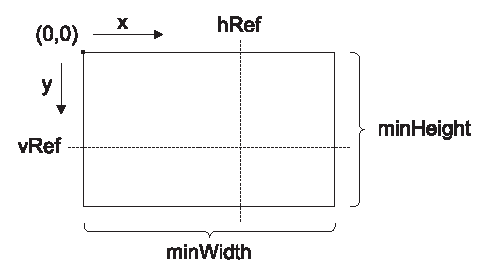
\includegraphics[width=2in]{images/PresentationBox}
\end{center}

A presentation tree in {Xprez} represents an attribute grammar with inherited and synthesized attributes. Presentation attributes that are typically specified for an entire subpresentation, such as color and font size, are inherited attributes.  \bc (going downward in the tree)\ec On the other hand, presentation attributes that are set by a child and used by its parent, such as  reference lines and size information, are synthesized attributes. Figure~\ref{xprezattributes} shows the two Haskell records  \p{Inh} and \p{Syn} that are used to model the inherited and synthesized presentation attributes. The figure also shows the type of each attribute. 

The \p{hRef} and \p{vRef} attributes specify the reference lines that are used for aligning boxes horizontally and vertically when combined in composite presentations. Note that the vertical-reference line is in fact a horizontal line and vice versa. The term vertical-reference line stems from the fact that it is used for vertical alignment; modifying the vertical-reference line affects the vertical position of the presentation. 

The boolean attributes \p{hStretch} and \p{vStretch} specify whether or not the presentation is allowed to stretch in horizontal or vertical direction. The remaining attributes are self-explanatory: \p{fontFamily}, \p{fontSize}, \p{textColor}, \p{lineColor}, \p{fillColor}, and \p{bgColor}. In the future, this set will be extended with other attributes such as line and font style, and attributes for modeling edit behavior (e.g.\ \p{onMouseClick~::~EditCommand}).
 
\bc
The presentation tree is transformed into an attribute grammar in which the font, style, and color properties are inherited attributes that go down in the tree, and alignment and stretch properties are synthesized attributes that go up in the tree. In the Haskell types, this division is visible in the fact that the properties are modeled using two records: \p{Inh} for inherited properties, and \p{Syn} for synthesized properties.
\ec

%																
\subsection{{\Xprez} primitives} \label{sect:primitives}

The first five combinators in Figure~\ref{xprezprim} specify atomic presentations. The \p{empty} combinator has a presentation that is invisible and takes up no space; it is the neutral element for various presentation compositions. A string is presented with combinator \p{text}, and a rectangle with combinator \p{rect}. The \p{poly} combinator takes a list of relative coordinates between (0.0, 0.0) and (1.0, 1.0) and produces a line figure that connects these points. The coordinates are relative because the final coordinates depend on the size of the \p{poly} presentation. Finally, \p{img} can be used to display external images. The argument is a string that contains the path to the image file. In a future version, an \p{img} term may also contain a reference to an image that is encoded as part of the document.

Except for \p{text}, the reference lines of an atomic presentation both have coordinate 0 (i.e.\ the north-west corner). For \p{text},  the vertical-reference line is the baseline of the text and the horizontal-reference line is at 0. By default, a  simple presentation does not stretch.

\begin{figure}
\begin{small}
\begin{center}
\begin{small}
\begin{verbatim}
empty             :: Xprez
text              :: String -> Xprez             
rect              :: Xprez                       
img               :: String -> Xprez             
poly              :: [ (Float, Float) ] -> Xprez 
row, col, overlay :: [ Xprez ] -> Xprez          
rowR, colR        :: Int -> [ Xprez ] -> Xprez   
matrix            :: [[ Xprez ]] -> Xprez
format            :: [ Xprez ] -> Xprez
\end{verbatim}
\end{small}
\caption{The {\Xprez} primitives} \label{xprezprim} 
\end{center}
\end{small}
\end{figure}

The remaining primitives in Figure~\ref{xprezprim} specify composite presentations. The behavior of columns (\p{col}) is equal to that of rows (\p{row}) with the horizontal and vertical directions swapped. Hence, we only discuss the \p{row} primitive. In a row, each child presentation is placed immediately to the right of its predecessor, with their vertical-reference lines aligned. Horizontal-reference lines have no effect on the positioning in a row.

\begin{center}
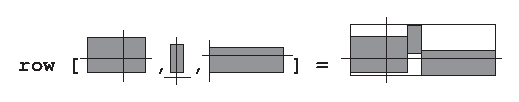
\includegraphics[width=3.2in]{images/row}
\end{center}

The bounding box of a row is the smallest rectangle that encloses all elements of the row. The vertical-reference line of the row is equal to the aligned reference lines of the children, whereas the horizontal-reference line is taken from the first child. In order to use the horizontal-reference line from one of the other children, we can use the \p{rowR} combinator. The integer argument of \p{rowR} specifies which child determines the horizontal-reference line for the row, with 0 denoting the first child. 

By default, a row stretches in horizontal direction if one of its children does, and it stretches in vertical direction if all children stretch vertically. The defaults may be overridden by setting the stretch attributes with the method that is  shown in the next section. 

The \p{matrix} combinator can be used to describe a table layout, in which elements are aligned with elements to their left and right as well as with elements above and below them. 

Because \p{row}, \p{column} and \p{matrix} do not allow their children to overlap, we need a special combinator for overlapping presentations. The \p{overlay} combinator places its children in front of each other, while aligning both the horizontal and vertical-reference lines. It can be used to create underlined text, for example. Because alignment takes place on both reference lines and hence all child reference lines overlap, no special \p{overlayR} combinator is needed.

A flow layout can be achieved with the \p{format} combinator for paragraph formatting. The combinator takes a list of presentations as argument and splits this list into rows based on the available horizontal space. The resulting rows are placed in a column.  Because \p{Xprez} does not yet have a page model, only horizontal formatting is supported. 

Here is an example {\Xprez} presentation that illustrates alignment and stretching in a row:

\begin{small}
\begin{verbatim}
let cross     = poly [(0,0),(1,0),(1,1),(0,1),(0,0),(1,1),(0,1),(1,0)]
    greycross = cross `withStretch` True `withbgColor` grey
in  row [ text "Big" `withFontSize` 200
        , colR 2 [ cross, cross, text "small", greycross, greycross ] ] 
\end{verbatim}
\end{small}

The code produces the following image (the dashed line has been added to show vertical-reference line of the presentation):

\begin{center}
\includegraphics[width=1in]{images/align}
\end{center}

The second element in the row is a column that takes the vertical-reference line from its third child. Therefore, the word ``Big'' is aligned with the word ``small''. The \p{cross} object is a line figure in the form of a rectangle with a cross. The \p{greycross} is a \p{cross}, which is made stretchable in both directions by \p{withStretch}, and which has a grey background.
 
Because the column contains presentations that stretch vertically, the column itself also stretches vertically. The column is created with a \p{colR} combinator with argument \p{2}, which causes the third child (\p{text "small"}) to be the object from which the reference lines of the column are taken.  The two stretching objects above the reference object are each assigned equal amounts of the remaining space above the vertical-reference line, and likewise, the objects underneath the reference object are assigned the remaining space below the reference line. If, on the other hand, the reference object itself is allowed to stretch, then the total amount of available space is distributed equally over all stretching objects. In this case, the reference object is not aligned. 

%																
\subsection{Modifying presentation attributes}

The presentation attributes of a presentation can be modified using the \p{with\symbol{95}} combinator. (The name has an underscore because ``\p{with}'' is a reserved word in Haskell.)

\begin{small}
\begin{verbatim}
with_ :: Xprez -> ((Inh, Syn) -> (Inh, Syn)) -> Xprez
\end{verbatim}
\end{small}

The combinator takes a single child presentation as argument, together with a function from attributes to attributes. The function is applied to the inherited attributes coming from the parent, and the synthesized attributes coming from the child. From the result of this application, the inherited attributes are passed to the child, whereas the synthesized attributes are passed to the parent. Thus, the \p{with\symbol{95}} combinator can be used to modify the inherited and synthesized attributes of a presentation.

\begin{figure}[t]
\begin{center}
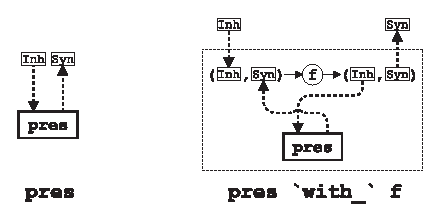
\includegraphics[width=6cm]{images/with}
\caption{Data flow for \p{with\symbol{95}}.}\label{withDataFlow} 
\end{center}
\end{figure}


Figure~\ref{withDataFlow} shows the data flow for the attributes of \p{pres} and \p{pres `with\symbol{95}` f}. Because \p{f} may be an arbitrary function, the combinator may introduce cycles in the attribution. It is up to the designer of the presentation to ensure safety.

Because the inherited and synthesized attributes are modeled as Haskell records, we use the Haskell record syntax for  accessing and updating presentation attribute values. Hence, for a record of inherited attributes \p{inh~::~Inh}, the expression \p{fontSize inh} denotes the value of the \p{fontSize} attribute in \p{inh}. Furthermore, \p{inh $\{$ fontSize = 10 $\}$} denotes a copy of \p{inh} in which the \p{fontSize} field is updated to 10. Thus, we can define a  \p{withFontSize} combinator: 

\begin{small}
\begin{verbatim}
withFontSize :: Xprez -> Int -> Xprez
withFontSize xp fs = xp `with_` \(inh, syn) -> (inh {fontSize = fs}, syn)
\end{verbatim}
\end{small}

The function argument to \p{with\symbol{95}} introduces a considerable syntactic overhead to the presentation code. To reduce this overhead, we can define a library of combinators, such as \p{withFontSize}, for frequent applications of  \p{with\symbol{95}}. Thus, most of the explicit applications of \p{with\symbol{95}} may be avoided.

Besides combinators that set an attribute value absolutely, we can also define combinators that take into account the original value of an attribute when setting its value. Consider the combinator \p{withFontSize\symbol{95}} defined below. Instead of an integer, it takes a function (\p{ffs~::~Int~->~Int}) as argument. Given the inherited font size, the function \p{ffs} specifies its new value.

\begin{small}
\begin{verbatim}
withFontSize_ :: Xprez -> (Int -> Int) -> Xprez
withFontSize_ xp ffs = 
  xp `with_` \(inh, syn) -> (inh { fontSize = ffs (fontSize inh) }, syn)
\end{verbatim}
\end{small}

With \p{pres `withFontSize\symbol{95}` (\symbol{92}fs -> 2*fs)} we specify that \p{pres} gets a doubled font size. An application of \p{withFontSize\symbol{95}} has a function argument, but the function is considerably simpler than the function argument of \p{with\symbol{95}}. 

The font-size combinators show how abstraction is used to meet the {\em proportional effort} requirement. For simple changes of the font size, the simple \p{withFontSize} combinator can be used, and only if more control is desired, it is necessary to use the more complicated \p{withFontSize\symbol{95}} or \p{with\symbol{95}} combinators.

A future version of {\Xprez} will support a domain-specific special syntax for \p{with\symbol{95}}. Thus, in order to specify that  a presentation \p{pres} gets twice the font size of its parent, a red background color, and a height that is twice the height of the letter `x' in the current font, we will be able to write something in the line of: 

\begin{small}
\p{pres\{ child.fontSize = 2*parent.fontSize, child.color = red, height = 1ex \}}
\end{small}%\nonote{niet duidelijk of ex voor ouderlijk of huidig font is}

%																
\subsection{Advanced examples} \label{sect:xprezFrac}

Because a presentation in {\Xprez} is a first-class value, it is possible to manipulate a child presentation (e.g.\ change its position or modify the font size) at the level of its parent.  This is illustrated in the presentation for a mathematical fraction: 


\begin{small}
\begin{verbatim}
frac e1 e2 = let numerator   = hAlignCenter (pad (shrink e1) )
                 bar         = hLine
                 denominator = hAlignCenter (pad (shrink e2) )
             in  colR 2 [ numerator, vSpace 2, bar
                        , vSpace 2, denominator ] `withHStretch` False

pad xp = row [ hSpace 2, xp, hSpace 2 ]

shrink e = e `withFontSize_` (\fs -> (70 `percent` fs) `max` 10)
\end{verbatim}
\end{small}

The non-primitive library function \p{hAlignCenter} centers its argument horizontally, and the \p{shrink} function reduces the font size to 70\%, with a minimum of 10. The result of \p{(text "x" `frac` text "2") `frac` text "1 + y"} is:

\begin{center}
\includegraphics[width=0.5cm]{images/frac}
\end{center}

The \p{pad} and \p{shrink} functions illustrate the {\em first-class} and {\em abstraction} requirements. Because a presentation is a first-class value, the presentations of the numerator and the denominator can be resized and positioned in the presentation of the fraction itself. Furthermore, we can abstract over positioning and resizing by using the functions \p{pad} and \p{shrink}. 

In contrast, child presentations in both P or PSL cannot be addressed at parent level. Hence, the numerator, the denominator, and even the fraction bar, each have to specify their own size and relative position. As a result, it is difficult to reuse parts of a presentation in another presentation, since all parts refer to each other. Furthermore, the manipulations on the appearance are harder to read, because no abstraction can be used. 

The second example is a pair of combinators that can be used to create tree-browser presentations:

\begin{center}
\includegraphics[width=1in]{images/tree}
\end{center}


The image has been created with the \p{mkTreeLeaf} and \p{mkTreeNode} combinators, shown in Figure~\ref{treeCombinators}. Both combinators take an \p{Xprez} argument that is the presentation of the label, and the tree node also takes a list of child presentations (which should be either nodes or leaves for a correct tree). A label is not restricted to text, but can be an arbitrary {\Xprez} presentation, as shown by the case statement at the bottom of the tree. The tree example shows that a complex and graphical presentation can be specified with relatively little effort. \todo{tree and frac in one figure, don't show tree code just say it's possible}


%%%%%%%%%%%%%%%%%%%%%%%%%%%%%%%%%%%%%%%%%%%%%%%%%%%%
%
\section{Presentation}
%
%%%%%%%%%%%%%%%%%%%%%%%%%%%%%%%%%%%%%%%%%%%%%%%%%%%%

\bl 
\o Ag for presentation and computing derived values/structures
\o each parsing parts specifies its parser, structural is automatic
\o example
\el


%%%%%%%%%%%%%%%%%%%%%%%%%%%%%%%%%%%%%%%%%%%%%%%%%%%%
%
\section{Scanning}
%
%%%%%%%%%%%%%%%%%%%%%%%%%%%%%%%%%%%%%%%%%%%%%%%%%%%%

\bl
\o What the scanner does:
\o on structural parts, put stuff in structural tokens, and recognize children
\o on parsing parts use scanner sheet to create tokens
\o result is Structural [.. [PresentationTk]..]
\o presentation is stored in these tokens
\o Alex
\o Example 
\o Automatic whitespace handling
\el
\bl
\o Explain layout layer somewhere
\o it adds layout explicitly, by looking it up in the map, and also restores the focus
\o if focus restore fails, focus is set on old coordinates (usually okay, explain when not)
\el
%%%%%%%%%%%%%%%%%%%%%%%%%%%%%%%%%%%%%%%%%%%%%%%%%%%%
%
\section{Parsing}
%
%%%%%%%%%%%%%%%%%%%%%%%%%%%%%%%%%%%%%%%%%%%%%%%%%%%%

\bl
\o structural vs parsing
\el

\bl
\o Structural: automatic
\o all information is encoded in the tree
\el

\bl
\o combinator parser
\o because of extra state (hidden presentations), and presentation ids, little bit extra info is kept
\o Example
\el


\bl
\o in case of parse error
\el

%%%%%%%%%%%%%%%%%%%%%%%%%%%%%%%%%%%%%%%%%%%%%%%%%%%%
%
\section{Incrementality(?)}
%
%%%%%%%%%%%%%%%%%%%%%%%%%%%%%%%%%%%%%%%%%%%%%%%%%%%%


%%%%%%%%%%%%%%%%%%%%%%%%%%%%%%%%%%%%%%%%%%%%%%%%%%%%
%
\section{Related work}
%
%%%%%%%%%%%%%%%%%%%%%%%%%%%%%%%%%%%%%%%%%%%%%%%%%%%%

\todo{more?}

\head{Eclipse}

Eclipse~\cite{eclipse2001} is a Java-based platform for building integrated development environments. The platform has an open architecture, and can be easily extended through a plug-in mechanism. Eclipse includes a syntax-recognizing Java editor, which supports in-place type information, refactoring, as well as document-oriented edit operations. 

Though it is not exactly a generic editor, Eclipse does have facilities for creating syntax-recognizing source editors. Unfortunately, building a code editor similar to the Java editor for a different language, requires a substantial amount of programming. Moreover, the presentation of the code is rather limited (lines of text), and there is no support for derived values appearing in the presentation.

\head{Barista, Citrus}

Barista~\cite{KoMyers06Barista} is a powerful framework for building code editors. It is built on top of Citrus~\cite{KoMyers05Citrus}, which is a UI toolkit together with an object-oriented language. Although Barista is targeted at code editors, the presentation of the code can be visual, for example allowing for images to appear in comments, or having graphical presentations of code. The editors created with Barista are syntax directed, but presentation-oriented editing is available. 

Because of the orientation towards code editing, word-processing editors will be harder to specify in Barista. The same holds for editors for which the structure of the presentation does not follow the structure of the document. Barista has no special support for derived values in the presentation or for editable derived structures.



%%%%%%%%%%%%%%%%%%%%%%%%%%%%%%%%%%%%%%%%%%%%%%%%%%%%
%
\section{Conclusion} 
%
%%%%%%%%%%%%%%%%%%%%%%%%%%%%%%%%%%%%%%%%%%%%%%%%%%%%

\bl
\o dtd pres and parser give simple environment
\o use ag to add static/type checks
\el

%%%%%%%%%%%%%%%%%%%%%%%%%%%%%%%%%%%%%%%%%%%%%%%%%%%%
%
% References

\bibliographystyle{sbc}
\bibliography{../proxima}

\end{document}
